\chapter{Sierpinski Triangle}

\noindent \\ Trekëndëshi i Sierpinskit është një fraktal i famshëm i emëruar pas matematikanit Waclaw Sierpinski. Fraktali mund të konstruktohet duke filluar nga një trekëndësh barabrinjësh dhe pastaj rekursivisht duke ndarë çdo trekëndësh si vijon:

\begin{enumerate}
    \item Në secilën brinjë të trekëndëshit gjejë pikën e mesit dhe bashkoj këto pika, ku formohen katër trekëndësha të rinjë.
    \item Përsërit procesin në secilin trekëndësh përveç trekëndëshit të mesëm.
\end{enumerate}

\noindent Katër iterimet e para të fraktalit janë paraqitur në figurën \ref{fig:sierpinski_iterations}. Me rritjen e iterimeve do të fitohet figura \ref{fig:sierpinski_big}.

\begin{figure}[htbp]
\hfill
\subfigure[Iterimi 0]{\includegraphics[width=0.24\linewidth]{triangle_1}}
\hfill
\subfigure[Iterimi 1]{\includegraphics[width=0.24\linewidth]{triangle_2}}
\hfill
\subfigure[Iterimi 2]{\includegraphics[width=0.24\linewidth]{triangle_3}}
\hfill
\subfigure[Iterimi 3]{\includegraphics[width=0.24\linewidth]{triangle_4}}
\hfill
\caption{Iterimet e para të fraktalit.}
\label{fig:sierpinski_iterations}
\end{figure}


\section{Konstruktimi i trekëndëshit të mbrendshëm}

Le të jetë dhënë trekëndëshi \( \triangle ABC \) dhe pikat \( D, E, F \) që përgjysmojnë brinjët e trekëndëshit (figura \ref{fig:triangle_construction}). Kordinatat e pikave \( D, E, F \) janë:


\[ D = \left( \frac{a_1 + b_1}{2}, \frac{a_2 + b_2}{2} \right) \]
\[ E = \left( \frac{b_1 + c_1}{2}, \frac{b_2 + c_2}{2} \right) \]
\[ F = \left( \frac{a_1 + c_1}{2}, \frac{a_2 + c_2}{2} \right) \]

\noindent \\ Trekëndëshat \( \triangle ADF \), \( \triangle DBE \), \( \triangle FEC \), do të hyjnë në iterimin e ardhshëm për ndarje.

\begin{figure}
    \centering
    \includegraphics[width=0.55\linewidth]{triangle_5.png}
    \caption{Konstruktimi i trekëndëshit të mbrendshëm.}
    \label{fig:triangle_construction}
\end{figure}

\section{Numri i pikave të figurës}

Në vizualizim të fraktalit, do të renderohet trekëndëshi fillestar me ngjyrë të gjelbërt dhe trekëndëshat e mbrendshëm me ngjyrë të zezë. Nevoitet të gjendet numri i pikave të trekëndëshave të mbrendshëm (të zi). Shënojmë me \( T(n) \) numrin e trekëndëshave që shtohen nga iterimi \( n-1 \) në \( n \). Pra në \( T(1) = 1 \), \( T(2) = 3 \), \( T(3) = 9 \). Secili trekëndësh pas ndarjes jep 3 trekëndësha të rinj në të cilët do konstruhohen trekëndëshat e zi.

\[ 
T(n) = 3T(n-1) = 3^2 T(n-2) = \cdots = 3^{n-1} T(1) = 3^{n-1} 
\]

\noindent \\ Numri i të gjithë trekëndëshave të zi në iterimin \(n\)  është shuma:
\[
T(1) + T(2) + \cdots + T(n) = 3^0 + 3^1 + \cdots + 3^{n-1} = \sum_{i=0}^{n-1} 3^i = \frac{3^n - 1}{2}
\]
\noindent Secili trekëndësh ka tre pika, dhe nëse llogarisim edhe 3 pikat e trekëndëshit fillestar kemi

\[
f(n) = 3 + \frac{3 \cdot (3^n - 1)}{2} = 3 + \frac{3^{n+1} - 3}{2} = \frac{3}{2} (3^n + 1)
\]

\noindent  Vargu \(f(n)\) paraqet numrin e të gjithë pikave të trekëndshave të brendshëm dhe të trekëndëshit fillestar në iterimin \(n\). Fillimisht kemi vizualisuar trekëndëshin inicializues me ngjyrë të gjelbërt (rreshti 6), dhe pastaj trekëndëshat e zi në rreshtin 10. \\ 

\begin{lstlisting}
void renderTriangleFromBuffer() {
 glVertexAttribPointer(0, 2, GL_FLOAT, GL_FALSE, 0, nullptr);
 glEnableVertexAttribArray(0);
 //Render first green triangle
 glColor3f(0.29f, 0.44f, 0.55f);
 glDrawArrays(GL_TRIANGLES, 0, 3);
 //Render blackTriangles
 int numberVerticesBlackTriangles = (pow(3, iterations + 1) - 3) / 2;
 glColor3f(0.0f, 0.0f, 0.0f);
 glDrawArrays(GL_TRIANGLES, 3, numberVerticesBlackTriangles);
 glutSwapBuffers();
} 
\end{lstlisting}


\section{Paralelizimi}

Paralelizimi ndodh në menyrë hiearkike, ku në secilin iterim do të jenë aktiv një numër i caktuar i thredave. Secili thread aktiv do e marë trekëndëshin e \(i\) -të të figurës, dhe do i gjejë tre pikat për ndërtimin e trekëndëshit të mbrendshëm. Tre trekëndëshat që do të ndahen në iterimin e ardshëm, definohen nga secili thread dhe futen në vargun e të gjithë trekëndëshave. Madhësia e këtij vargu do të jetë numri i pikave të trekëndëshave të gjetur në formulën në raport me 3, sepse secili trekëndësh ka tri pika.

\[
\frac{f(n)}{3} = \frac{1}{2} (3^n + 1)
\]



\noindent \\ Për secilin iterim do të jenë \(3^n\) threada aktiv. Me rritje të iterimeve, numri i thredave aktiv do të ngirtet eksponencialisht:
\begin{itemize}
    \item Iterimi 0: Vetëm threadi me id 0 të jetë aktiv. Ky thread inicalizon trekëndëshin fillestar.
    \item Iterimi 1: Vetëm threadi me id 1 është aktiv. Ky thread ndërton trekëndëshin e parë të mbrendshëm. Tre trekëndëshat definohen dhe futen në vargun e trekëndëshave në pozitat 2,3,4, të cilët do ndahen në iterimin e ardhshëm.
    \item Iterimi  2: Threadat 2,3,4 janë aktiv. Secili thread mer trekëndëshin përkatës në bazë të indeksit të tyre. Secili thread ndërton trekëndëshin e mbrendshëm, definon 3 trekëndëshat, të cilët futen në vargun e të gjithë trekëndëshave.
    \item Iterimi \(n\): Threadat \(\frac{3^n + 1}{2}\) deri në \(\frac{3^{n+1} - 1}{2}\) do të jenë aktiv. Këta threada marrin trekëndëshat nga iterimi i kaluar dhe ndërtojnë trekëndëshat e mbrendshëm në ta.
\end{itemize}

\begin{figure}[]
    \centering
    \includegraphics[width=0.3\linewidth]{triangle_6.png}
    \caption{Nyja me fëmijë në graf ternar.}
    \label{fig:node_ternary}
\end{figure}

\begin{figure}[htpb]
    \centering
    \includegraphics[width=1\linewidth]{triangle_7.png}
    \caption{Sinkronizimi dhe ekzekutimi paralel.}
    \label{fig:sierpinski_parallel}
\end{figure}

\noindent \\ Paralelizimi dhe shtimi i të dhënave është modeluar në një graf ternar si në figurën \ref{fig:sierpinski_parallel}. Çdo nyje në graf ternar përfaqëson një thread që ndërton trekëndëshat e mbrendshëm, ndërsa degët përfaqësojnë ndarjen e tre trekëndëshave në iteracionet e ardhshme. Secili thread \(i\)  merr trekëndëshin \(i\) nga vargu i trekëndëshave, e ndan atë, dhe shton tre trekëndësha të ri në pozitat  fëmijë \(3i-1,3i,3i+1\) (figura \ref{fig:node_ternary}). Secili nivel i grafit përfaqëson threadat të cilët janë duke punuar në paralel. 

\noindent \\ Indeksi më i djathtë i nivelit \(n\) të grafit është pikërisht shuma:
\[
\text{rightMost}(n) = \sum_{i=0}^n 3^i = \frac{3^{n+1} - 1}{2}
\]
\noindent Indeksi më i majtë i nivelit \(n\) të grafit është:
\[
\text{leftMost}(n) = \text{rightMost}(n-1) + 1 = \frac{3^n - 1}{2} + 1 = \frac{3^n + 1}{2}
\]
\noindent Numri i thredave që punojnë në paralel në nivelin \(n\):
\[
\text{leftMost}(n+1) - \text{leftMost}(n) = \frac{3^{n+1} + 1}{2} - \frac{3^n + 1}{2} = 3^n
\]

\section{Kerneli}

Kerneli i mëposhtëm gjeneron fraktalin përmes llogaritjes paralele. Fillimisht threadi me indeks 0 trajton trekëndëshin inicializues. Për secilin iterim threads ndërmjet intervalit start\_at dhe end\_at janë aktiv dhe llogaritin meset e segmenteve të trekëndëshit. Definohen tri trekëndësha të rinjë të cilët ruhen në vargun e trekëndshëva që do të ndahen. Meset e segmenteve i shtohen vargut points për vizualizim të trekëndëshit. Sinkronizimi siguron që të gjitha threadat përfundojnë detyrën e tyre para sa te të vazhdojnë në iterimin e ardhshëm.  \\

\begin{lstlisting}
__global__ void kernel(float* points, Triangle* triangles, int start_iteration, int max_iteration, int threadShiftIndex) {
    int idx = threadIdx.x + blockDim.x * blockIdx.x;
    idx += threadShiftIndex;
    Point A,B,C,A1,B1,C1;
    Triangle triangle,t_1,t_2t_3;
    auto g = cg::this_grid();
    if (idx == 0) {
    triangles[1] = triangle;
    }
    
    for (int iteration = start_iteration; iteration <= max_iteration; iteration++) {
        int start_at = (round((pow(3, iteration) + 1))) / 2;
        int end_at = (round((pow(3, iteration+1) - 1))) / 2;
        if (idx >= start_at && idx <= end_at) {
            triangle = triangles[idx];
            A = triangle.A;
            B = triangle.B;
            C = triangle.C;
            //DivideTriangle 
            A1.x = (A.x + B.x) / 2.0f;
            A1.y = (A.y + B.y) / 2.0f;
            B1.x = (B.x + C.x) / 2.0f;
            B1.y = (B.y + C.y) / 2.0f;
            C1.x = (C.x + A.x) / 2.0f;
            C1.y = (C.y + A.y) / 2.0f;
            //Make three new Triangles
            t_1.A = A;
            t_1.B = A1;
            t_1.C = C1;
            
            t_2.A = A1;
            t_2.B = B;
            t_2.C = B1;
            
            t_3.A = C1;
            t_3.B = B1;
            t_3.C = C;
            //Insert three new triangles to triangles array
            triangles[3 * idx - 1] = t_1;
            triangles[3 * idx] = t_2;
            triangles[3 * idx + 1] = t_3;
            
            //Add three points 
            int offset = 2 * 3 * (idx);
            points[offset] = A1.x;
            points[offset + 1] = A1.y;
            points[offset + 2] = B1.x;
            points[offset + 3] = B1.y;
            points[offset + 4] = C1.x;
            points[offset + 5] = C1.y;
        }
        g.sync();
    }
}

\end{lstlisting}


\section{Krahasimet}

Tabela \ref{tab:sierpinski_table} krahason kohën e ekzekutimit në mikrosekonda të fraktalit ndërmjet versionit sekuencial dhe të versionit paralel. Implementimi me CUDA është bërë me  anë të grupeve kooperative, me 25600 threada për një thirrje të kernelit. Vizualizimi i këtyre rezultave është në figurën \ref{fig:sierpinski_graph}.

\begin{table}[h]
\centering
\resizebox{0.4\textwidth}{!}{%
\begin{tabular}{|l|l|l|}
\hline
Iterimi & C++ & CUDA( \\ \hline
0 & 1 & 32 \\ \hline
1 & 2 & 23 \\ \hline
2 & 3 & 23 \\ \hline
3 & 3 & 31 \\ \hline
4 & 5 & 20 \\ \hline
5 & 19 & 23 \\ \hline
6 & 47 & 19 \\ \hline
7 & 133 & 23 \\ \hline
8 & 257 & 22 \\ \hline
9 & 861 & 37 \\ \hline
10 & 2633 & 34 \\ \hline
11 & 8374 & 82 \\ \hline
12 & 30457 & 243 \\ \hline
13 & 74373 & 653 \\ \hline
14 & 271835 & 1886 \\ \hline
15 & 1060085 & 6367 \\ \hline
16 & 5812052 & 2782181 \\ \hline
17 & 14557977 & 6679207 \\ \hline
\end{tabular}
}
\caption{Krahasimi i performancës.}
\label{tab:sierpinski_table}
\end{table}



\begin{figure}[h]
\centering
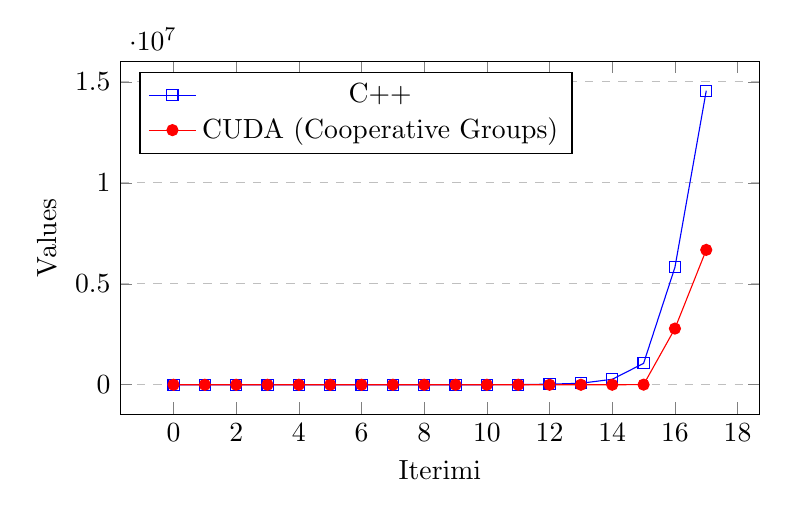
\begin{tikzpicture}
\begin{axis}[
    title={},
    xlabel={Iterimi},
    ylabel={Values},
    legend pos=north west,
    ymajorgrids=true,
    grid style=dashed,
    width=0.8\textwidth,  % Adjust width as needed
    height=0.5\textwidth, % Adjust height as needed
]
\addplot[
    color=blue,
    mark=square,
    ]
    coordinates {
    (0,1)(1,2)(2,3)(3,3)(4,5)(5,19)(6,47)(7,133)(8,257)(9,861)(10,2633)(11,8374)(12,30457)(13,74373)(14,271835)(15,1060085)(16,5812052)(17,14557977)
    };
\addplot[
    color=red,
    mark=*,
    ]
    coordinates {
    (0,32)(1,23)(2,23)(3,31)(4,20)(5,23)(6,19)(7,23)(8,22)(9,37)(10,34)(11,82)(12,243)(13,653)(14,1886)(15,6367)(16,2782181)(17,6679207)
    };
\legend{C++, CUDA (Cooperative Groups)}
\end{axis}
\end{tikzpicture}
\caption{Grafiku i krahasimit të performancës.}
\label{fig:sierpinski_graph}
\end{figure}


\newpage


\begin{figure}[]
    \centering
    \makebox[\textwidth]{\includegraphics[width=1.8\linewidth]{triangle_8.png}}
    \caption{Trekëndëshi i Sierpinskit në iterimin 7 i gjeneruar me CUDA.}
    \label{fig:sierpinski_big}
\end{figure}

